\documentclass[a4paper]{report}
\usepackage{tikz}
\begin{document}
\pagestyle{empty}
\begin{center}
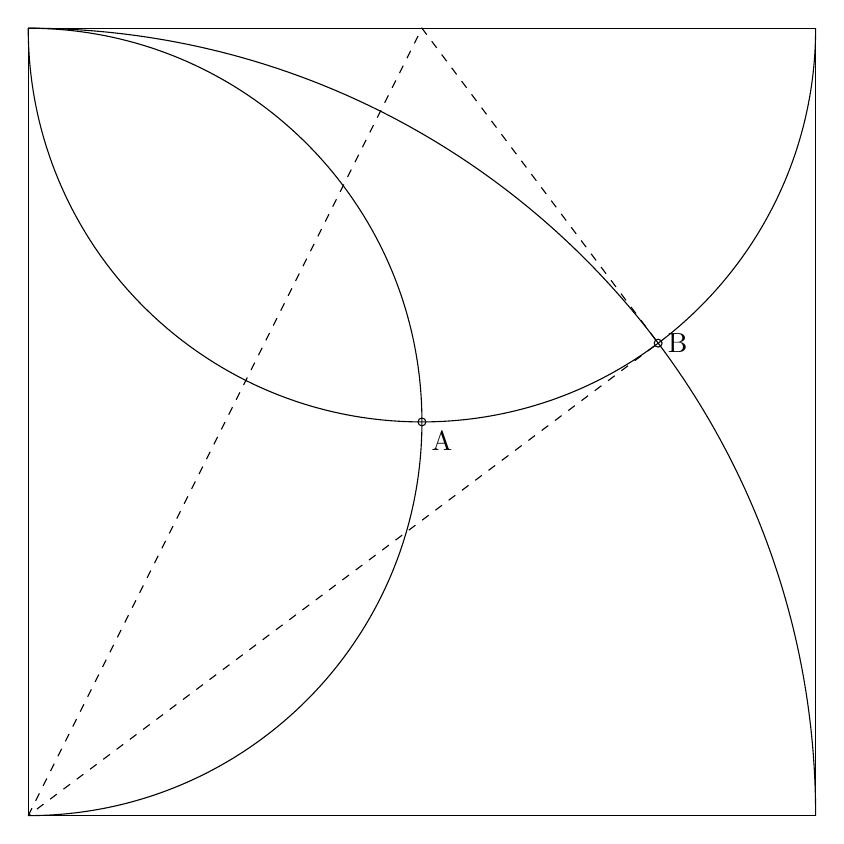
\begin{tikzpicture}
\coordinate (B) at (8,6);
\coordinate (A) at (5,5);
\draw (0,0) rectangle (10,10);
\draw  (10,0) arc (0:90:10);
\draw (0,0) arc(-90:90:5); 
\draw (0,10) arc (180:360:5);
\draw (A) circle (0.5mm) node [below right]{A};
\draw (B) circle (0.5mm) node [right]{B};
\draw [dashed](0,0)--(5,10)--(B)--(0,0);
\end{tikzpicture}
\end{center}
Primero encontramos el punto más importante. que es el punto $B$ 

\end{document}